I\chapter{Results}
\label{cha:results}

This chapter reports the results of several real world instances of Makahiki implemented in different organizations, as well as the the application of SGSEAM to the Makahiki framework.

\section{Real World Case Studies}

We have used Makahiki to create totally seven (7) Kukui Cup Energy Challenges in four different organizations. The following sections describes the Makahiki instances for the four organizations and the different configurations between these instances.

\subsection{University of Hawaii at Manoa}

There are three instances of Kukui Cup Challenges implemented by using the Makahiki framework in the university of Hawaii at Manoa (UHMM). They are held in 2011, 2012, and 2014 respectively for over 1000 first year students living in the residence halls on campus. The three instances have different competition durations, which are 3 weeks, 9 months and 2 weeks respectively. The residence halls where the students living in have energy smart meters installed for collecting the real time energy data consumed by the students. 

\begin{figure}[ht!]
   \centering
   \includegraphics[width=20em]{uhm-homepage}
   \caption{UHM Kukui Cup Challenge Home Page}
   \label{fig:uhm-homepage}
\end{figure}

%% TODO: describe the general feedback of the challenge

\subsection{Hawaii Pacific University}

There are two instances of Kukui Cup Challenges implemented by using the Makahiki framework in the Hawaii Pacific University (HPU). They are held in 2012 and 2013 respectively for about 200 students living in the residence halls at the Hawaii Loa Campus. Energy smart meters were installed in the residence halls.

\begin{figure}[ht!]
   \centering
   \includegraphics[width=20em]{hpu-homepage}
   \caption{HPU Kukui Cup Challenge Home Page}
   \label{fig:hpu-homepage}
\end{figure}

\subsection{East-West Center}

The EWC Kukui Cup Energy and Water challenge was implemented by an international organization called the East-West Center (EWC) using the Makahiki framework. It was held in 2013 for approximately 600 international students living in their residence halls in Hawaii. The challenge lasts for 2 weeks and includes energy and water saving competition between two residence halls. The residence halls did not have internet-enabled smart meters.

\begin{figure}[ht!]
   \centering
   \includegraphics[width=20em]{ewc-homepage}
   \caption{EWC Kukui Cup Challenge Home Page}
   \label{fig:ewc-homepage}
\end{figure}

\subsection{Holy Nativity School}

A pilot instance of Kukui Cup challenge implemented by using the Makahiki framework was held at the Holy Nativity School (HNS), a private elementary school in Hawaii, in 2013. The pilot instance was organized by the school with the partnership with Project Learning Tree (PLT) GreenSchool! program\cite{plt-greenschools}. The nationwide environmental service-learning program helps improve students’ academic performance in STEM subjects by engaging students in STEM as they solve environmental issues at their school.

\begin{figure}[ht!]
   \centering
   \includegraphics[width=20em]{hns-homepage}
   \caption{HNS Kukui Cup Challenge Home Page}
   \label{fig:hns-homepage}
\end{figure}

\subsection{Customization of the Makahiki Instances}

The following sections describe the different customizations that were done to the above Makahiki instances according to the different organizations' needs.

\subsubsection{Configuration Customization}
The challenge configuration includes the duration of the challenge, the participant accounts, resource such as energy and water settings, learning action configurations, prize and other game mechanics settings. 

\autoref{table:challenge-configurations} lists the different configurations between the seven real world instances of Makahiki.

\begin{table}[ht!]
  \centering
  \begin{tabular} {|c|c|c|c|c|c|c|c|c|}
    \hline
    \tabhead{Instances} &
    \tabhead{Participants} &
    \tabhead{Teams} &
    \tabhead{Duration} &
    \tabhead{Rounds} &
    \multicolumn{4}{c|}{\tabhead{Game Element}} \\
    \cline{6-9}
    & & & & &     
    \tabhead{Energy} &
    \tabhead{Water} &
    \tabhead{Prize} &
    \tabhead{Quest} \\
    \hline
    UHM2011 & 1000 & 20 & 3 weeks & 3 & \checkmark & \xmark & \checkmark & \checkmark\\
    \hline
    UHM2012 & 1086 & 20 & 9 months & 4 & \checkmark & \xmark & \checkmark & \checkmark\\
    \hline
    UHM2014 & 1093 & 20 & 2 weeks & 2 & \checkmark & \xmark & \checkmark & \checkmark\\
    \hline
    HPU2012 & 190 & 6 & 3 weeks & 3 & \checkmark & \xmark & \checkmark & \checkmark\\
    \hline
    HPU2013 & 190 & 6 & 3 weeks & 3 & \checkmark & \xmark & \checkmark & \checkmark\\
    \hline
    EWC2012 & 130 & 2 & 2 weeks & 1 & \checkmark  & \checkmark & \xmark & \xmark\\
    \hline
    HNS2013 & 10 & 2 & 4 weeks & 1 & \xmark & \xmark & \checkmark & \checkmark \\
    \hline
  \end{tabular}
  \caption{Challenge Configuration Differences}
  \label{table:challenge-configurations}
\end{table}

As we can see from the \autoref{table:challenge-configurations}, the Makahiki framework can be customized to support different size of the team competition with different duration, with energy, water and both competition, as well as the different education contents of
the sponsoring organizations. For example, while UHM and HPU
challenges involved only energy consumption data, the EWC challenge involved both energy
and water consumption data. 

\subsubsection{Content Customization}
Because the different organizations have different sustainability educational needs, they used the Makahiki framework to customize the content, which is shown to student players via the SmartGrid Game mechanics. They can re-use or modify the existing contents came with the Makahiki framework or create new content to be included in the system. The \autoref{table:sgg-configurations} shows the difference in the type and layout of the educational contents. UHM had the most number of the learning actions while HNS has the least. 

\begin{table}[ht!]
  \centering
  \begin{tabular} {|c|c|c|c|c|c|c|}
    \hline
    \tabhead{Instances} &
    \tabhead{Levels} &
    \tabhead{Activities} &
    \tabhead{Commitments} &
    \tabhead{Events} & 
    \tabhead{Total Actions}\\
    \hline
    UHM2011 & 1 & 51 & 21 & 21  & 93 \\
    \hline
    UHM2012 & 7 & 68 & 23 & 35  & 126 \\
    \hline
    UHM2014 & 4 & 60 & 21 & 20  & 101\\
    \hline
    HPU2012 & 3 & 24 & 11 & 4  & 39 \\
    \hline
    HPU2013 & 3 & 29 & 11 & 4  & 44 \\
    \hline
    EWC2012 & 4 & 21 & 1 & 19  & 41 \\
    \hline
    HNS2013 & 2 & 22 & 6 & 4  & 32 \\
    \hline
  \end{tabular}
  \caption{Content Differences}
  \label{table:sgg-configurations}
\end{table}

The layout of the educational content represented in the SmartGrid game is also highly customizable to include different levels, rows and columns. The figures  \autoref{fig:UHM-SGG}, \autoref{fig:HPU-SGG}, \autoref{fig:EWC-SGG}, \autoref{fig:GS-SGG} illustrate the content and layout of the educational SmartGrid game in the different Makahiki instances. 

\begin{figure}[http]
	\centering
		\subfigure[UHM 2011 Kukui Cup SmartGrid Game]{\label{fig:uh-2011}\includegraphics[height=3.6in,width=3.5in]{UH-SGG-2011.eps}}
		\subfigure[UHM 2012 Kukui Cup SmartGrid Game]{\label{fig:uh-2012}\includegraphics[height=1.8in,width=3.5in]{UH-SGG-2012.eps}}
		\subfigure[UHM 2014 Kukui Cup SmartGrid Game]{\label{fig:uh-2014}\includegraphics[height=1.8in,width=3.5in]{UH-SGG-2014.eps}}
		\caption{UHM SmartGrid Game Layouts}
		\label{fig:UHM-SGG}
\end{figure}

\begin{figure}[htbp]
	\centering
		\subfigure[HPU SmartGrid Game Level1]{\label{fig:hpu-level1}\includegraphics[height=2in,width=3.5in]{HPU-SGG-level1.eps}}
		\subfigure[HPU SmartGrid Game Level2]{\label{fig:hpu-level2}\includegraphics[height=2in,width=3.5in]{HPU-SGG-level2.eps}}
		\subfigure[HPU SmartGrid Game Level3]{\label{fig:hpu-level3}\includegraphics[height=2in,width=3.5in]{HPU-SGG-level3.eps}}
		\caption{HPU SmartGrid Game Layouts}
		\label{fig:HPU-SGG}
\end{figure}

\begin{figure}[htbp]
	\centering
		\subfigure[EWC SmartGrid Game Level1]{\label{fig:ewc-level1}\includegraphics[height=1.7in,width=3.5in]{EWC-SGG-level1.eps}}
		\subfigure[EWC SmartGrid Game Level2]{\label{fig:ewc-level2}\includegraphics[height=1.7in,width=3.5in]{EWC-SGG-level2.eps}}
		\subfigure[EWC SmartGrid Game Level3]{\label{fig:ewc-level3}\includegraphics[height=1.7in,width=3.5in]{EWC-SGG-level3.eps}}
		\subfigure[EWC SmartGrid Game Level4]{\label{fig:ewc-level4}\includegraphics[height=1.7in,width=3.5in]{EWC-SGG-level4.eps}}
		\caption{EWC SmartGrid Game Layouts}
		\label{fig:EWC-SGG}
\end{figure}

\begin{figure}[htbp]
	\centering
		\subfigure[HNS SmartGrid Game Level1]{\label{fig:gs-level1}\includegraphics[height=2in,width=3.5in]{GS-SGG-level1.eps}}
		\subfigure[HNS SmartGrid Game Level2]{\label{fig:gs-level2}\includegraphics[height=2in,width=3.5in]{GS-SGG-level2.eps}}
		\caption{HNS SmartGrid Game Layouts}
		\label{fig:GS-SGG}
\end{figure}

\subsubsection{Branding Customization}
The look and feel of the challenges website are difference between the different organizations, which is customized using the customization feature of the Makahiki framework. The user interface was customized to ``brand'' each challenge. The list of customizable branding are:

\begin{itemize}
\item logo
\item size name
\item challenge name
\item team label
\item landing page text
\item about page text
\item sponsor text and logo
\item theme
\end{itemize}

\subsubsection{System Configuration}

The system configuration includes the infrastructure hosting, user authentication, and smart meter connections. 

\autoref{table:system-configurations} lists the different configurations between the seven real world instances of Makahiki.

\begin{table}[ht!]
  \centering
  \begin{tabular} {|c|c|c|c|c|c|c|}
    \hline
    \tabhead{Instances} &
    \tabhead{Hosting} &
    \tabhead{Authentication} &
    \tabhead{Smart meters} \\
    \hline
    UHM2011 & Local & CAS & \checkmark \\
    \hline
    UHM2012 & Cloud & CAS & \checkmark \\
    \hline
    UHM2014 & Cloud & CAS & \checkmark \\
    \hline
    HPU2012 & Local & LDAP & \checkmark \\
    \hline
    HPU2013 & Local & LDAP & \checkmark \\
    \hline
    EWC2012 & Cloud & CAS \& Internal & \xmark \\
    \hline
    HNS2013 & Cloud & Internal & \xmark \\
    \hline
  \end{tabular}
  \caption{System Configuration Differences}
  \label{table:system-configurations}
\end{table}
 
UH and HPU used different metering infrastructure, and EWC collected their resource data manually.  Since the
halls did not have internet-enabled meters, resource consumption data had to be entered by
the game managers manually.

The IT infrastructure at UH and HPU provided
authentication services using CAS (Central Authentication Service) and LDAP, while EWC
used the built-in Django authentication.  

\section{SGSEAM assessment}

The successful creation of serious game challenges by four different organizations
provides evidence that Makahiki can be successfully tailored to the needs of different organizations. This section describes the result of applying a formal assessment method of SGSEAM to the Makahiki framework to assess the strengths and weaknesses of the Makahiki as a serious game framework.

The \autoref{fig:assessment-overview} provides the overview of applying SGSEAM to Makahiki.

\begin{table}[ht!]
  \centering
  \begin{tabular}{|p{0.2\columnwidth}|p{0.4\columnwidth}|p{0.2\columnwidth}|}
    \hline
    \tabhead{Stakeholder} &
    \tabhead{Assessment Approach} &
    \tabhead{Experiments}  \\
    \hline
    \multirow{4}{*}{Players} & Pre Post effectiveness study & \multirow{4}{*}{UHM KC} \\
    \cline{2-2}
     & Self-reported effectiveness survey &  \\
    \cline{2-2}    
     & Self-reported usability survey &  \\
    \cline{2-2}
     & Engagement metrics &  \\
    \hline
   \multirow{2}{*}{System admins} & In-lab installation study & ICS691 \\
    \cline{2-3}
     & Post-hoc system admin interview & HPU KC \\
    \hline
   \multirow{2}{*}{Game designers} & In-lab game design study & ICS691 \\
    \cline{2-3}
     & Post-hoc game designer interview & HPU \& EWC KC \\
    \hline
   \multirow{2}{*}{Game managers} & In-lab game management study & ICS691 \\
    \cline{2-3}
     & Post-hoc game manager interview & HPU \& EWC KC \\
    \hline
   Developers & In-lab game development study & ICS691 \\
    \hline
  \end{tabular}
  \caption{SGSEAM assessments for Makahiki}
  \label{fig:assessment-overview}
\end{table}

\subsection{Makahiki Player Assessment}

We used four approaches to assess the player experience for the Makahiki framework. They are pre-post effectiveness study, self-report effectiveness survey, self-report usability survey, and engagement metrics. The real world Makahiki instances of UHM Kukui Cup challenge were used for the Makahiki player assessments. 

\subsubsection{Pre Post effectiveness study}

In the 2011 Kukui Cup Challenge at the University of Hawaii at Manoa, a serious game implemented using the Makahiki framework, there were over 1000 eligible players for this challenge, who were mostly first
year college students living in the 5 resident halls. The challenge was designed to lasted for 3 weeks and the student players are divided into 20 teams based on the dorm locations where they resided, each team's energy consumption is measured a smart meter installed in the various locations inside the resident hall. Makahiki recorded the energy consumption for the players before, during and after the challenge. Makahiki also recorded detailed logging data from every interaction between the players and the website. 

To assess the effectiveness of the framework for designing games that improve player literacy in sustainability, 
 two energy literacy surveys were conducted, one before the challenge (pre-game) and one after
the challenge (post-game). 

Robert Brewer designed and conducted the survey. The results are reported in his dissertation \cite{csdl2-10-08}. 24 players completed both surveys. Out of the total 19 energy literacy questions, the average number of questions answered correctly is 7.54 before the
challenge, and 8.96 after the challenge. This result indicates an 18\% improvement on the
energy literacy.  Non-players as a control condition were also surveyed. The result is shown in the \autoref{fig:UHM-literacy-result}. According to Brewer \cite{csdl2-10-08}, ``Based on the questionnaire results, it appears that the energy knowledge of challenge participants increased modestly compared to those that did not participate in the challenge.''.
\begin{figure}[ht!]
  \center
  \includegraphics[width=0.9\columnwidth]{UHM-literacy-result}
  \caption{Literacy Survey Result of UHM 2011 KC from Robert Brewer 's Dissertation \cite{csdl2-10-08}}
  \label{fig:UHM-literacy-result}
\end{figure}

To assess the effectiveness of the framework for designing games that produce positive change in sustainability
behaviors, The energy consumption data that collected before, during and after the
challenge were used to compare the differences.  Before the challenge, an energy usage baseline was established. 

Robert Brewer calculated the energy consumption data before and after the UHM 2011 Kukui Cup challenge. According to his dissertation \cite{csdl2-10-08}, 12 out of the total 20 teams reduced their energy
consumption compared to the baseline. The highest reduction of 16.1\%. However, 3 teams actually increased
their energy consumption, with the highest increase of 11.7\%. Overall, the average
reduction of the 20 teams was approximately 2\%.  The result is shown in the \autoref{fig:UHM-energy-result}. 
\begin{figure}[ht!]
  \center
  \includegraphics[width=0.9\columnwidth]{UHM-energy-result}
  \caption{Energy Consumption Result of UHM 2011 KC from Robert Brewer's Dissertation \cite{csdl2-10-08}}
  \label{fig:UHM-energy-result}
\end{figure}

Sara Cobble \cite{csdl2-12-14} from Hawaii Pacific University conducted the similar energy consumption study on the 2012 HPU Kukui Cup instance. Her result, as shown in \autoref{fig:HPU-energy-result}, shows that one team met the energy reduction goal (which is 5\%) for 14 days out of the 3 weeks competition, with an average 11.3\% energy reduction. The average numbers of days meeting the reduction goal for all the teams is 6.5 days, with an average energy reduction of 5.1\%.

\begin{figure}[ht!]
  \center
  \includegraphics[width=0.75\columnwidth,height=1.7in]{HPU-energy-result}
  \caption{Energy Reduction Result of HPU 2012 KC from Sara Cobble's Report \cite{csdl2-12-14}}
  \label{fig:HPU-energy-result}
\end{figure}

In summary, the SGSEAM can provide evidences of the Makahiki achieving literacy improvement and some positive change in
behavior.

\subsubsection{Self-reported effectiveness survey}
A survey to gather the opinions of participants regarding the effect of the challenge to their sustainability behavior was included at the last round of the challenge. 
Two survey questions was used to assess the self-reported perception of the players regarding the interests in energy conservation and sustainability prior and after playing the Kukui Cup. 

In the 2011 UHM Kukui Cup challenge, 43 players completed the survey. The responses to the survey are in free text. We analyzed the free text responses and coded them into three categories: ``Yes'', ``No'', and ``Somewhat''. \autoref{table:interests-in-sustainability} lists results of the responses. \autoref{fig:effect-prior-after} illustrates the percentages of self-reported interests in the sustainability prior to the KuKui Cup and the effect after playing the Kukui Cup.

\begin{table}[ht!]
  \centering
  \begin{tabular} {|p{0.6\linewidth}|c|c|c|}
    \hline
    \tabhead{\multirow{2}{*}{Question}} & \multicolumn{3}{c|}{\tabhead{Number of Responses}} \\
    \cline{2-4}
    \tabhead{} & \tabhead{Yes} & \tabhead{No } & \tabhead{Somewhat}\\
    \hline
    Prior to playing the Kukui Cup, were you interested in energy conservation? & 24 & 8 & 11\\
    \hline
    Has the Kukui Cup increased your interest in energy conservation and sustainability?& 37 & 0 & 6 \\
    \hline
  \end{tabular}
  \caption{Interests in sustainability prior and after the KC (2011 UHM, n=43)}
  \label{table:interests-in-sustainability}
\end{table}

\begin{figure}[htbp]
	\centering
		\subfigure[interests in sustainability prior]{\label{fig:effect-prior}\includegraphics[height=2.2in]{effect-prior.eps}}
		\subfigure[increased interests in sustainability after]{\label{fig:effect-after}\includegraphics[height=2.2in]{effect-after.eps}}
		\caption{Interests in sustainability prior and after the UHM 2011 KC}
		\label{fig:effect-prior-after}
\end{figure}

The self-reported responses indicates that there are a small percentage (19\%) of players were not interested in the sustainability prior to the Kukui Cup. After playing the Kukui Cup, 100\% of responses reported an affirmative or somewhat increase of interests in sustainability. 

In 2012 UHM Kukui Cup challenge, the similar survey questions were included the last round. 44 players completed both the two questions. \autoref{table:interests-in-sustainability-2012} lists results of the responses. \autoref{fig:effect-prior-after-2012} illustrates the percentages of self-reported interests.

\begin{table}[ht!]
  \centering
  \begin{tabular} {|p{0.6\linewidth}|c|c|c|}
    \hline
    \tabhead{\multirow{2}{*}{Question}} & \multicolumn{3}{c|}{\tabhead{Number of Responses}} \\
    \cline{2-4}
    \tabhead{} & \tabhead{Yes} & \tabhead{No } & \tabhead{Somewhat}\\
    \hline
    Prior to playing the Kukui Cup, were you interested in energy conservation? & 28 & 4 & 12\\
    \hline
    Has the Kukui Cup increased your interest in energy conservation and sustainability?& 37 & 5 & 2 \\
    \hline
  \end{tabular}
  \caption{Interests in sustainability prior and after the KC (2012 UHM, n=44)}
  \label{table:interests-in-sustainability-2012}
\end{table}

\begin{figure}[htbp]
	\centering
		\subfigure[interests in sustainability prior]{\label{fig:effect-prior-2012}\includegraphics[height=2.2in]{effect-prior-2012.eps}}
		\subfigure[increased interests in sustainability after]{\label{fig:effect-after-2012}\includegraphics[height=2.2in]{effect-after-2012.eps}}
		\caption{Interests in sustainability prior and after the 2012 UHM KC}
		\label{fig:effect-prior-after-2012}
\end{figure}

The self-reported responses from 2012 KC indicates that there are a smaller percentage (9\%) of players than 2011 KC that were not interested in the sustainability prior to the Kukui Cup. After playing the Kukui Cup, 89\% of responses reported an affirmative or somewhat increase of interests in sustainability. There are 5 players (11\%)  reported that there is no changes of interests in sustainability. A closer look at the data indicates that the 5 players that reported no changes of interests also answered ``Yes'' or ``Somewhat'' interested to the sustainability prior to the Kukui Cup. The 4 players that reported no interests in sustainability also reported that playing KC had increased their interests.

The followings are some sample responses from the students who considered the Kukui Cup had increased their interests in sustainability:
 
 \begin{itemize}
 \item Yes. I'm more aware of everything I am using.
\item I've been interested, but the Kukui Cup has expanded and broadened my mind on what else I can be doing to help with conservation and sustainability. I think people are genuinely concerned, they just don't know how to exactly conduct them, or what other ways they can do it.
\item Yes, it made me realize that you can save a lot of money by turning off and unplugging a few things. (Hopefully lower tuition? =D )
\item It has increased my interest since I didn't know much about how much energy were using.
\item Some workshops made me think differently of how I use energy. Makes alternatives more interesting for me.
\item It taught me some new interesting facts about renewable energy and made me more aware.
\end{itemize}

There was a question in the 2011 KC survey tasking about the players' perception about how would they describe the Kukui Cup. The players were asked to check all that applies to their agreement to the following descriptions of the Kukui Cup: Educational, Fun, Addictive, So-so, Difficult, Boring, Not useful, and Other where they will type in their free text response. There were 43 responses from the 2011 KC survey. The number of responses and their percentage are listed in the \autoref{table:how-is-kc}.

\begin{table}[ht!]
  \centering
  \begin{tabular} {|c|c|c|}
    \hline
    \tabhead{Question: How would you describe the Kukui Cup?} & \tabhead{Number of Responses} & \tabhead{Percentage}\\
    \hline
Educational	& 41 & 95\%\\
    \hline
Fun	& 39 & 91\% \\
    \hline
Addictive	 &19 & 44\%\\
    \hline 
So-so	& 9 & 21\%\\
    \hline
difficult	& 3 & 7\%\\
    \hline
Boring	& 1 & 2\%\\
    \hline
not useful	& 0 & 0\\
    \hline
Other & 5 & 12\%\\   
    \hline 
  \end{tabular}
  \caption{Self-reported Perception of the Kukui Cup in 2011 UHM KC (n=43)}
  \label{table:how-is-kc}
\end{table}
	
Majority of the responses indicated the players perceived the Kukui Cup as ``Educational'' (95\%) and ``Fun'' (91\%). There are 44\% players perceived Kukui Cup as ``Addictive". On the other hand, there are 1 player (2\%) considered the Kukui Cup as``Boring". The ``Other'' responses are: ``AWSOME-NESS''(1), ``engaging''(1), ``fun competition''(1), ``Great way to bond with others''(1), ``impressive''(1).

A survey question was also asked about the players' self reported behavior change during the challenge in the 2012 UHM Kukui Cup. The question is ``Did you change your behavior during the competition based on the commitment(s) you made? if so, how?". It is a free response question. 45 players completed the survey in the 2012 UHM KC. I categorized the free text responses into three categories: ``Yes'', `already a habit'', and ``no''. The results are listed in \autoref{table:behavior-change}.

\begin{table}[ht!]
  \centering
  \begin{tabular} {|p{0.5\linewidth}|c|c|}
    \hline
    \tabhead{Question: Did you change your behavior during the competition based on the commitment(s) you made?} & \tabhead{Number of Responses} & \tabhead{Percentage}\\
    \hline
Yes	& 39 & 87\%\\
    \hline
Already a habit	& 4 & 9\% \\
    \hline
No	 &2 & 4\%\\
    \hline 
  \end{tabular}
  \caption{Self-reported Behavior Changes in 2012 UHM KC (n=45)}
  \label{table:behavior-change}
\end{table}

The examples of a ``Yes'' response are:
\begin{itemize}
\item ``I changed my behavior during the commitments but found myself doing the same things i did before after they were over.''
\item ``Yes, because knowing the facts of how much energy we use has helped me realize that I have been wasting money and energy.''
\item ``yes, my behavior has changed during the competition. I'm more aware of the things i do such as turning off appliances when not in use, as well as using more natural energy such as sunlight, rather than electricity.''
\end{itemize}

A ``Already a habit'' response is that the commitments already become part of the daily habit. The examples are:
\begin{itemize}
\item ``Most of the commitments I made I already did.''
\item ``I always turn off my lights when I leave the room, use cold water to wash my clothes, and I lessen my meat intake. ''
\end{itemize}

The self-reported survey results indicate in general, the players of Makahiki considered their experiences are positive and there had some self-reported impacts to their sustainability behaviors. 

\subsubsection{Self-reported usability survey}

A survey to gather the opinions of players regarding the usability of the website was added during the last round of the challenge. 

The players were asked to rate how much you agree with the following 4 usability statements in a likert scale (Strongly disagree, Disagree, Neutral, Agree, Strongly agree):
\begin{enumerate}
\item ``It was easy to find what I was looking for in the website.''
\item ``The website was responsive. I did not wait too long after I clicked on something.''
\item ``The website provided adequate help in teaching me how to play the game.''
\item ``I understood the rules of the game and how to play.''
\end{enumerate}

The questions were asked in both the 2011 and 2014 Kukui Cup in the University of Hawaii at Manoa, 43 players completed the survey in the 2011 KC while 18 players completed in the 2014 KC.  

\autoref{table:self-report-usability-2011}  and \autoref{table:self-report-usability-2014}  lists the results of the self-reported usability responses for both 2011 and 2014 Kukui Cup at UHM.

\begin{table}[ht!]
  \centering
  \begin{tabular} {|p{0.42\linewidth}|P{0.09\linewidth}|p{0.09\linewidth}|p{0.075\linewidth}|p{0.06\linewidth}|P{0.09\linewidth}|}
    \hline
    \centering \tabhead{Usability statement} & \tabhead{Strongly disagree} & \tabhead{Disagree} & \tabhead{Neutral} & \tabhead{Agree} & \tabhead{Strongly agree}\\
    \hline
It was easy to find what I was looking for in the website.& 2 & 1 & 2 & 14 & 24 \\
    \hline
The website was responsive. I did not wait too long after I clicked on something.& 2 & 1 & 1& 19 & 20 \\
    \hline
The website provided adequate help in teaching me how to play the game.	 & 1 & 1 & 1 & 16 & 24\\
    \hline
I understood the rules of the game and how to play	& 1& 1 & 0 & 12 & 29\\
    \hline 
  \end{tabular}
  \caption{Self-reported Usability in 2011 UHM KC (n=43)}
  \label{table:self-report-usability-2011}
\end{table}

\begin{table}[ht!]
  \centering
  \begin{tabular} {|p{0.42\linewidth}|P{0.09\linewidth}|p{0.09\linewidth}|p{0.075\linewidth}|p{0.06\linewidth}|P{0.09\linewidth}|}
    \hline
    \centering \tabhead{Usability statement} & \tabhead{Strongly disagree} & \tabhead{Disagree} & \tabhead{Neutral} & \tabhead{Agree} & \tabhead{Strongly agree}\\
    \hline
It was easy to find what I was looking for in the website.& 0 & 0 & 1 & 9 & 8\\
    \hline
The website was responsive. I did not wait too long after I clicked on something.& 0 & 4 & 2 & 10 & 2 \\
    \hline
The website provided adequate help in teaching me how to play the game.& 0 & 0 & 2 & 10 & 6 \\
    \hline
I understood the rules of the game and how to play.& 0 & 0 & 1 & 10 & 7 \\
    \hline 
  \end{tabular}
  \caption{Self-reported Usability in 2014 UHM KC (n=18)}
  \label{table:self-report-usability-2014}
\end{table}

\autoref{fig:self-report-usability-2011-2014} illustrates the self-reported usability measurements in both 2011 KC and 2014 KC. Majority of players reported that they agreed that the usability of the website is good with one exception of responsiveness from the 2014 responses. 4 out of 18 players (22\%) of 2014 KC reported that they considered the website is not very responsive. Comparing to the result of the 2011 KC, this indicates that there may be a perceived performance downgrade in the 2014 KC website.

\begin{figure}[ht!]
	\centering
		\subfigure[2011 Self-reported Usability Measurements(n=43)]{\label{fig:self-report-usability-2011}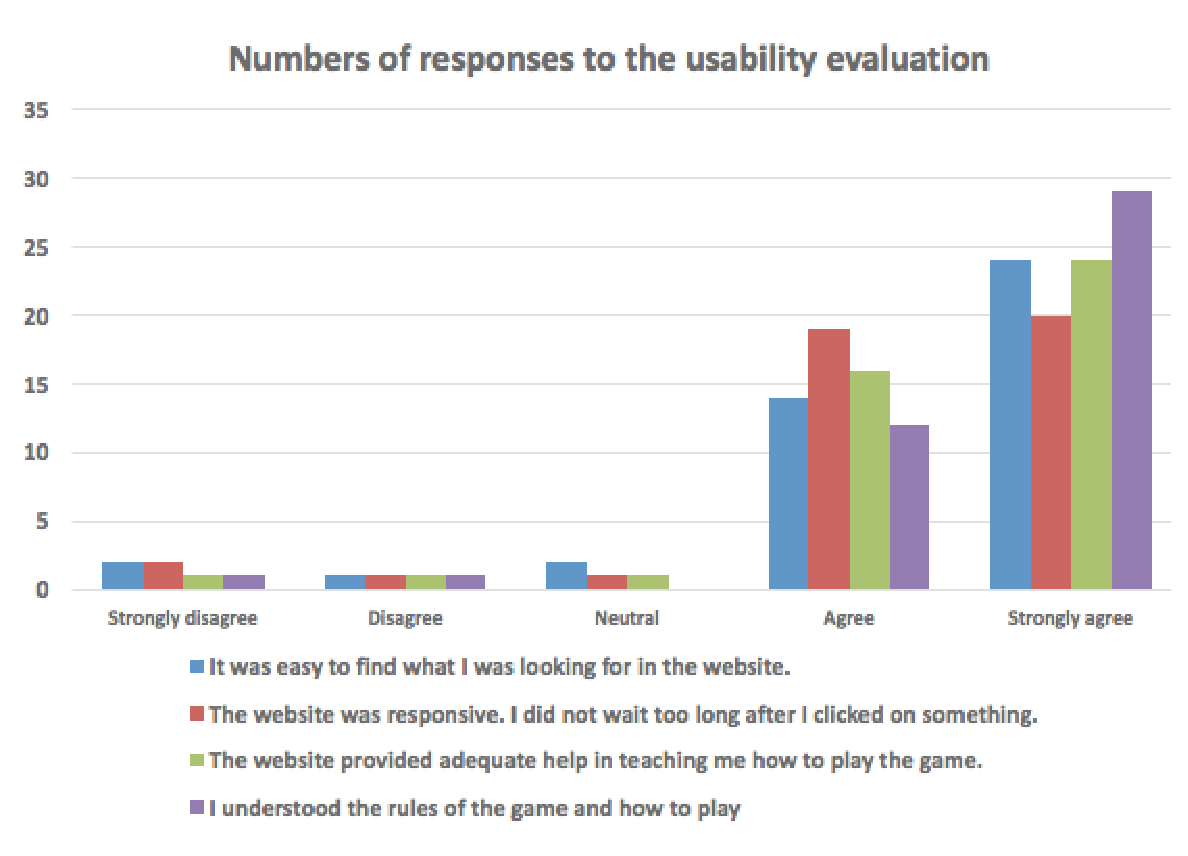
\includegraphics[height=3in]{self-report-usability-2011.eps}}
		\subfigure[2014 Self-reported Usability Measurements(n=18)]{\label{fig:self-report-usability-2014}\includegraphics[height=3in]{self-report-usability-2014.eps}}
		\caption{Self-reported Usability Measurements in 2011 KC and 2014 KC}
		\label{fig:self-report-usability-2011-2014}
\end{figure}

Another question was asked in the 2014 UHM KC survey regarding the issues encountered when playing using the website. There are 3 out of 18 responses (17\%) reported that the loading of the website page were slow. This confirms the responsiveness issues discovered in the self-reported usability measurements described above. Another issues reported in the responses to the survey question is the confusion of the scoreboard display in the website. 3 out of 18 responses (17\%) reported that scoreboard's display keep changing so it is not easy to see their rankings. There are also 2 responses reported that some of the videos were not displayed which is due to the links to the videos were outdated.

In summary , the self-reported usability survey is a good tool to get feedback from the players of Makahiki to reveal the strengths and weaknesses regarding the usability of the game. 

\subsubsection{Engagement metrics}

Based on the engagement metrics \ref{Engagement metrics} proposed in the SGSEAM, we calculated a variety of engagement metrics to assess the player's engagement level in the Kukui Cup challenge created by the Makahiki framework. The metrics are calculated by analyzing the website logs and the data collected by the website. The results shown in \autoref{fig:makahiki-engagement} are the engagement metrics for the 2011 Kukui Cup challenge at the University of Hawaii at Manoa.
    
\begin{table}[ht!]
  \centering
  \begin{tabular}{|p{0.3\linewidth}|c|c|c|c|c|c|}
    \hline
    \tabhead{\multirow{2}{*}{Measurement}} & \multicolumn{3}{c|}{\tabhead{2011 KC}} & \multicolumn{3}{c|}{\tabhead{2012 KC}}\\
     \cline{2-7}
    \tabhead{} & \tabhead{MIN} & \tabhead{AVG} & \tabhead{MAX} &  \tabhead{MIN} & \tabhead{AVG} & \tabhead{MAX}\\

    \hline
    Participation rate & 13\% & 37\% & 74\% & 19\% & 34\% & 64\%\\
    \hline
    Number of players per day & 43 & 85 & 147 & 0 & 12 & 130 \\
    \hline
    Play time per day & 1 min & 27.7 mins & 8.5 hours & 0 & 6.2 mins & 8.8 hours\\
    \hline
    Submissions per day & 32 & 266 & 1110 & 0 & 30 & 953\\
    \hline
    Social interactions per day & 51 &  208 & 468 & 0 & 31 & 502\\
    \hline
    Website errors per day & 0 & 0.6 & 4 & 0 & 2 & 458\\
    \hline
  \end{tabular}
  \caption{Engagement Metrics for 2011 and 2012 UHM Kukui Cup}
  \label{fig:makahiki-engagement}
\end{table}

The participation rate is the percentage of players who played the game. The 2011 UHM KC had a 37\% average participation rate, while the 2012 KC had 34\%. Both are good compared to other sustainability challenges. 

Over the 3 weeks course of the challenge in the 2011 KC, an average player spent about 27.7 minutes per day on the website, while in the 24 weeks challenge in 2012 KC, an average player spent about 6.2 minutes per day. Both instances had one player spent over 8 hours (8.5 and 8.8 respectively) on one day, which is quite significant amount of time for a student to spent in this kind of game. The daily minimum time spent on the 2011 KC is 1 minute which indicates that for every day during the challenge, there are at least one player who played at least 1 minute. The daily minimum time spent on the 2012 KC is 0 minutes. This indicates that there are at least one day when no player use the website.

In order to investigate the engagement in a more details, we looked at the engagement measurement in a time series format. \autoref{fig:timeseries-metrics} shows the timed measurements graph during the 2011 and 2012 Kukui Cup.

\begin{figure}[ht!]
  \center
  \includegraphics[height=3.2in,width=6in]{timeseries-metrics}
  \caption{Engagement Measurements during the 2011 and 2012 UHM Kukui Cup}
  \label{fig:timeseries-metrics}
\end{figure}

The divided line in the graphs indicates the division of the rounds for the 2011 and 2012 KC. In the 2011 KC, there are 3 rounds, each round lasted 1 week. In the 2012 KC, there are 4 rounds, the first and second round lasted 2 weeks each, and the third round lasted about 8 weeks, while the last round lasted about 12 weeks, with the total of 24 weeks for the 2012 KC. 

In addition to the daily number of players and daily play time which indicate the level of visits to the website or game, the daily submission and daily social interaction measurement indicate the level of deeper interactions with the game. We can see that during the 3 short weeks of the 2011 KC, the engagement patterns are similar in each week. The first few days has higher level of interactions then decreased later into the week. There is a spike on the last day of the round, which may be due to the urge of the players to check the winning results of the round. 

We can also see that in the 2012 KC, the engagement level significantly dropped after the second round, which is 4 weeks after the beginning of the game. There are still some numbers of players spent times on the game but the number of submissions and social interactions had decreased significantly. Over the time, the number of players decreased in the third round and even less in the last round. It is interesting to see that there are still some amounts of play time during the third and fourth round. A closer look at the data indicated that they are time spent from the the several top players who may be winning the game. 

Although the website error in the 2012 KC shown in the  \autoref{fig:makahiki-engagement} seems high, the detailed graph in \autoref{fig:timeseries-metrics} shows that the errors mostly happened during in one day which is the day after the start of the last round. The investigation of the error in the log file revealed that they are due to a content configuration error in a newly available event in the last round. The error caused the players not able to submit the completion of the event to claim their points so they kept trying and encountered the error repeatedly. The error was corrected 2 hours later after the first such error occurred.

In summary, SGSEAM indicates that Makahiki can be successful in achieving player engagement.

\subsection{Makahiki System Admin Assessment}
We used two approaches to assess the system administrators' experience with the Makahiki framework. They are in-lab installation study and post-hoc system admin interview.

\subsubsection{In-lab installation study}

In the in-lab installation study, the participants are the students in a serious game class (ICS691) in the Spring 2012 in the computer science department at the University of Hawaii at Manoa. The students were tasked with installing the Makahiki system into their local computers as well as deploying to the Heroku cloud environment. A Google Form was used to ask the students to record the time they spent completing each step and the problems they encountered. The students also provided feedback about their installation experiences in the form of blog posts. 

There were a total of 8 students who voluntarily participated in the experiments.  The participants were either senior undergraduates or graduate students majoring in Computer Science. The results from the Google Form responses show that the average total time to successfully install
Makahiki was 1.4 hours, with a maximum time of 2 hours and the minimum time of 0.9 hour.
\autoref{fig:install-time} shows the average time for each installation step.

\begin{figure}[ht!]
  \center
  \includegraphics[width=0.7\columnwidth]{install-time}
  \caption{Average time (minutes) for installation steps (n=8)}
  \label{fig:install-time}
\end{figure}

We coded and categorized the descriptive problems reported by the students in both the Google Form
and their blog posts. \autoref{fig:makahiki-install} shows the result of the analysis from
the feedback of the 8 students that participated in the experiment.

\begin{table}[ht!]
  \centering
  \begin{tabular}{|p{0.7\columnwidth}|c|}
    \hline
    \tabhead{Problem encountered} & \tabhead{Number of participants} \\
    \hline
    Cannot find configuration file to edit during database installation  & 4 \\
    \hline
    Documentation of install script is confusing about creation of the DB user & 2 \\
    \hline
    More parts of installation could be covered by install script & 2 \\
    \hline
  \end{tabular}
  \caption{Makahiki Installation Analysis (n=8)}
  \label{fig:makahiki-install}
\end{table}


From the above analysis, we identified that the ``Install and configure database'' step has the
longest average time. It is also has the most participant reported problems. This reflects the issues
encountered by students during the configuration process. This assessment determines the areas for future
improvement are (1) to improve documentation on DB installation, and (2) to improve the install script to automate
more installation tasks.

In summary, SGSEAM identified database installation as a weak point in
installation.  Otherwise, SGSEAM indicates generally positive results regarding
Makahiki with respect to installation.

\subsubsection{Post-hoc System Admin Interview}
In order to gain insights on the experience of a real world system admin who uses the Makahiki, I performed interviews to the system admins of the Hawaii Pacific University (HPU) Kukui Cup challenges and analyzed the problems encountered during the software installation and system administration. The HPU KC server software was installed by the system administrator from the HPU IT department with the assistances from us. The installation was performed in the HPU local IT infrastructure with the integration to the HPU LDAP server and their email server.  During the installation, issues encountered during the installation were communicated through emails and phone calls between the administrator and us. The interview took place after the challenge. The questions are outlined in the system admin assessment section of the SGSEAM. 

The data about the system admin experience was compiled and listed in \autoref{fig:makahiki-install-hpu2012} and \autoref{fig:makahiki-install-hpu2013} for the HPU KC instances for 2012 and 2013 respectively. The time to complete is the working days for the HPU system admin to complete the tasks reflected by the announcement in the email exchange and the conversation during the interview. During those working days, the system admin might have other work responsibilities not related to the Makahiki software installation. So the actual time to complete might be less.

\begin{table}[ht!]
  \centering
  \begin{tabular}{|P{0.28\columnwidth}|P{0.1\columnwidth}|p{0.5\columnwidth}|}
    \hline
     \tabhead{Installation Task} &
     \tabhead{Time to Complete} &
     \tabhead{Problem Encountered} \\
    \hline
     Install and startup & 5 days & error in installing the runtime environment virtualenvwrapper\\
    \hline
    Install image library & 1 day & error in displaying JPG image during testing \\
    \hline
     Use HPU LDAP server &  20 days &  need to install ldap libraries; need to create a special bind user to connect to the ldap server; use the correct ldap DN; HPU ldap server use non-standard way to identify user so the Makahiki software need to update to support HPU's server settings \\
    \hline
    Use HPU Email Server & 2 days & need to create a special email account for KC admin;  HPU email server reported error if the "from" parameter is not the same as the email account so the Makahiki software need to fix to support HPU's email. \\
    \hline
    Update the software & 1 day & none \\
    \hline
    Use SSL & not complete & need to procure the SSL certificate; the SSL certificate acquired by HPU does not have a trusted CA, it is decided that the competition will start without SSL \\
    \hline
    Total & 29 days & \\
    \hline
  \end{tabular}
  \caption{Installation Issues in HPU 2012 KC }
  \label{fig:makahiki-install-hpu2012}
\end{table}

\begin{table}[ht!]
  \centering
  \begin{tabular}{|P{0.28\columnwidth}|P{0.1\columnwidth}|p{0.5\columnwidth}|}
    \hline
     \tabhead{Installation Task} &
     \tabhead{Time to Complete} &
     \tabhead{Problem Encountered} \\
    \hline
     Startup from last year's Vmware image & 1 day &  none\\
    \hline
    Use HPU LDAP server & 1 day  & not able to login because the HPU LDAP server changed to use a new directory structure \\
    \hline
     Makahiki software upgrade & 1 day & need to recreated database migration script due to HPU still use older Postgresql DB version. \\
    \hline
     Use the new LDAP server &  1 day &  need to reconfigure to use the new LDAP server\\
    \hline
    Use HPU Email Server & 2 days & not able to send email because the HPU email server configuration change. \\
    \hline
    Total & 6 days & \\
    \hline \end{tabular}
  \caption{Installation Issues in HPU 2013 KC }
  \label{fig:makahiki-install-hpu2013}
\end{table}

The data shows that the the configuration to use HPU's LDAP server and email server are the most difficult tasks. It took a comparable large amount of time to install the ldap libraries, create the ldap account, testing the correct configuration and eventually discovered that the Makahiki software need to modify to support HPU's special server settings. 

Once the integration with the HPU's local infrastructure was completed in 2012, the 2013 experience is much easier, the LDAP and email server configuration changes was able to completed shortly in 2013.

When asked about the experience in maintaining the Makahiki server, such as backup and monitoring, the system admin answered that it is fairly straightforward to perform  the backup.  Since the server was built on the VMWare virtual machine, he used the built-in VMWare snapshot function to perform the daily backup. The backed up image was successfully used in 2013 as the starting point for the 2013 KC instance without the need to re-install the software. The system admin did not do any monitoring and relied on the game designer and manager to report any issues to him. During the running period of the two challenges, there is no report on the performance issues. Only one issue reported by the game designer during the testing is related to the system installation, that is the JPG image support library not being installed.

%%%% TODO in summary, and talk about the system interface change, impact

\subsection{Makahiki Game Designer Assessment}

\subsubsection{In-lab game design study}

We also used the in-lab experiment to assess the game
designer experience of Makahiki. One of the class assignments for the students in the
experiment was to design a serious game using the Makahiki framework. We asked the students
to follow specific design steps and record the time required and any problems encountered during
their design process, using a Google Form similar to the one used for the system admin
assessment. In addition, students were asked to provide feedback about their
design experiences in the form of blog posts. \cite{csdl2-13-04} describes in detailed
the Google Form that is used in this assessment.

The game designer assessment was generalized into 7 tasks corresponding to
distinct types of administrative tasks and game design planning. The time for each task is
calculated from the Google Form results.  

There were a total of 8 students who voluntarily participated in the experiments. The most time consuming task is "Smart Grid Game Design", which took average 107.9 minutes (56\% of total time) to complete, while the least time consuming tasks is "Raffle Game Design", which took average 7.9 minutes (7\% of total time) to complete.

\autoref{fig:design-time} shows the average time for each design tasks:

\begin{figure}[ht!]
  \center
  \includegraphics[width=0.7\columnwidth]{design-time}
  \caption{Average time (minutes) for design tasks (n=8)}
  \label{fig:design-time}
\end{figure}

 We aggregated the problems reported in the feedback of the 8 students that participated in the experiment.
\autoref{fig:makahiki-game-design} shows the result of the analysis:

\begin{table}[ht!]
  \centering
  \begin{tabular}{|p{0.7\columnwidth}|c|}
    \hline
    \tabhead{Problem encountered} &
    \tabhead{Number of participants} \\
    \hline
    Difficulty in understanding predicate system and unlock condition & 7 \\
    \hline
    A bug that prevented users with usernames containing capital letters from logging in & 2 \\
    \hline
    A bug in the processing of Ajax queries & 1 \\
    \hline
    Difficulty in generating event attendance codes for game activities & 1 \\
    \hline
  \end{tabular}
  \caption{Makahiki Game Design Analysis, (n=8)}
  \label{fig:makahiki-game-design}
\end{table}

In summary, SGSEAM revealed two shortcomings with Makahiki configuration: ``Smart
Grid Game Design'' and ``Configure Challenge Settings''. Issues encountered in ``Smart Grid Game
Design'' included 1) difficulty and lack of documentation on the predicate system used to define dependencies
between game activities, and 2) difficulty in generating event attendance codes for game activities.
Issues encountered in ``Configure Challenge Settings'' included 1) a bug in the processing of Ajax queries
caused by consecutive clicks on the same interface button, and 2) a bug that prevented users with username
containing capital letters from logging in.

\subsubsection{Post-hoc Game Designer Interview}
In order to gain insights on the experience of a real world game designer who uses the Makahiki software to design the serious game, I performed interviews to the game designer of the two Kukui Cup challenges in Hawaii Pacific University (HPU) and East West Center (EWC) in the year of 2012. The game designer for HPU is the sustainability coordinator for the Hawaii Pacific University; while the game designers for EWC are two sustainability coordinator for the East-West Center Participant Association. We asked them about their game designing experiences using the Makahiki game design interface. The interview questions are outlined in the game design section of the SGSEAM. In addition to the interview data, Makahiki system log file and email exchanges were analyzed to identify the problems encountered during the game design process.

\autoref{fig:hpu-design} and \autoref{fig:ewc-design} lists the game design experience with Makahiki for the 2012 HPU and 2012 EWC Kukui Cup instances respectively. 

\begin{table}[ht!]
  \centering
  \begin{tabular}{|P{0.5\columnwidth}|P{0.4\columnwidth}|}
    \hline
    \centering \tabhead{Problem encountered} &  \tabhead{Cause} \\
    \hline
    Error displaying the prize page after adding a prize  & Makahiki software did not validate the prize parameter inputted \\
    \hline
    The introduction video referenced to previous year &  The introduction video should be made generic so it could be reused over years \\
    \hline
    Error when users save their profile in the profile page & Python Image Library is not installed correctly\\
    \hline
    Confusion of the event code generation & The admin interface to generate the event code is not intuitive\\
    \hline
    Don't know how to creating external link in Kukui Cup Activities description & The markup language for activity description is not WYSIWYG \\
    \hline
    Smartgrid layout not change immediately after the settings changed & The cache is not clear automatically when setting changed\\
    \hline
  \end{tabular}
  \caption{Makahiki Game Design Experiences in 2012 HPU Kukui Cup}
  \label{fig:hpu-design}
\end{table}

\begin{table}[ht!]
  \centering
  \begin{tabular}{|P{0.5\columnwidth}|P{0.4\columnwidth}|}
    \hline
    \centering \tabhead{Problem encountered} & \tabhead{Cause} \\
    \hline
    confusing in generating the confirmation code  & the admin interface is not intuitive \\
    \hline
    don't know how to use video other than youtube &  Makahiki software only support youtube video id \\
    \hline
    forget to change the default commitment period & the default is meant for testing and not typical\\
    \hline
    not able to delete the FAQ widget from help page & the admin interface to find the name of the widget on a page is not intuitive \\
    \hline
  \end{tabular}
  \caption{Makahiki Game Design Experiences in 2012 EWC Kukui Cup}
  \label{fig:ewc-design}
\end{table}

One EWC designer responded that ``It is easy to create the smartgrid game, putting the video etc. The interface is easy to use.''. She also mentioned that ``Just a little bit time consuming.''

\subsection{Makahiki Game Manager Assessment}
In order to gain insights on the experience of a real world game designer who uses the Makahiki software to design the serious game, I performed interviews to the game manager of the two Kukui Cup challenges in Hawaii Pacific University (HPU) and East West Center (EWC) in the year of 2012. The game manager for HPU is the sustainability coordinator for the Hawaii Pacific University; while the game managers for EWC are two sustainability coordinator for the East-West Center Participant Association. They are also the game designers for their Kukui Cup instances. We asked them about their game management experiences using the Makahiki admin
interface. The interview questions are outlined in the game manager section of the SGSEAM. We also analyzed the Makahiki instance log file and email exchanges between the game managers and us to identify the problems encountered during the game management process.

\autoref{fig:hpu-ewc-manage} lists the game management experience with Makahiki for the 2012 HPU and 2012 EWC Kukui Cup instances. 

\begin{table}[ht!]
  \centering
  \begin{tabular}{|P{0.4\columnwidth}|P{0.4\columnwidth}|P{0.1\columnwidth}|}
    \hline
    \centering \tabhead{Problem encountered} &
    \centering \tabhead{Cause} & 
    \tabhead{Reporting Instance} \\
    \hline
    not easy to find the event confirmation code  & the admin interface to view the event confirmation code is not intuitive & HPU and EWC \\
    \hline
    error when click on the "save and add another" button in the approval admin interface, the "save" button is ok &  the approval admin interface should remove the "save and add another" button & HPU and EWC \\
    \hline
    some status data disappear after the competition ended & Makahiki software bug & HPU\\
    \hline
    missing two days worth of energy and water data & did not enter the manual energy and water data in time & EWC\\
    \hline
    Intermittently unable to access the website  & there was an DNS problem with the domain name registrar & EWC\\
    \hline
  \end{tabular}
  \caption{Makahiki Game Managing Experiences in 2012 HPU and EWC Kukui Cup}
  \label{fig:hpu-ewc-manage}
\end{table}

When asked if it was easy to approve the player's submissions, HPU manager responded that it was ``very easy''. 

About the approval process, HPU game manager responded that he made sure that player submissions were either approved or rejected
within 12 hours. He also discovered a useful feature in the approval interface without
help from the Makahiki support team. 

EWC game managers responded with more issues during the game managing process, as discussed in the followings:
\begin{itemize}
\item participation game does not make sense since the total number of residences are different

\item a hassle to manually enter the data;

\item have to manually sign up user before and during the game

\item hard to choose the appropriate points for various competing elements

\item Adjusting the point system in the middle of the game cause potential unfairness

\item need to make the game site available to player after the competition over. software not support yet, EWC admin worked around it by extending the game for one more week

\item did not support sending out email daily to inform the progress or current status of the game.  software not support yet. EWC admin worked around by manually sending out the status email
\end{itemize}

In summary, SGSEAM uncovered few problems with Makahiki game management using the interview
approach. We realized that the confident level of this assessment approach is low because of
 availability of only one data point. An experimental study approach or perform interviews to
multiple game managers will increase the confidence level of the assessment.

\subsection{Makahiki Developer Assessment}

We assessed developer experience using an in-lab experiment. In the ICS691 serious game development class, the participating students were asked to complete the assignment to develop an enhancement to Makahiki.  This involved setting up a development environment, following the tutorial to create a ``Hello World'' widget using Makahiki, and finally, developing enhancements to extend the functionality of Makahiki which include 5 required development tasks.  The students were asked to submit their development source code to the public source code repository (GitHub) and write a blog post to discuss their efforts and experiences in completing the development activities. The estimated completion time is 10 to 30 hours. The students were told to complete as much as possible and if not complete, they should report in the blog post that what part is not complete. The blog posting should also discuss the parts of the enhancement exercise that they found easy to complete, the parts they found hard to complete, and their recommendations for how the Makahiki framework could be improved to support such enhancement activities more easily in the future. 

The \autoref{table:makahiki-dev} lists the results of the development status after analyzing the blog posts and the source codes they submitted to GitHub. 

\begin{table}[ht!]
  \centering
  \begin{tabular}{|p{0.5\columnwidth}|c|c|}
    \hline
    \tabhead{Development Task} &
    \tabhead{Number of completion} & 
    \tabhead{Reported Difficulty}\\
    \hline
    Setup development env & 8 & easy\\
    \hline
    Create the ``Hello World'' widget & 8 & easy\\
    \hline
    Update score\_mgr class to support groups. & 7 & easy \\
    \hline
    Create a group scoreboard widget. & 7 & a little hard \\
    \hline
    Create a group resource widget. & 4 & hard\\ 
     \hline
    Create a group prize widget. & 2 & hard\\
     \hline
    Create two group statistics widgets for the status page & 1 & hard\\
    \hline
  \end{tabular}
  \caption{Makahiki Game Development Experience, (n=8)}
  \label{table:makahiki-dev}
\end{table}

All 8 students reported that the first three tasks of setting up the environment, creating the  ``Hello world'' widget and extending the score\_mgr class was easy, while the rest of the enhancements was hard. Only one student was able to successfully
completed all required enhancement developments, while the most of them was able to  successfully completed the reported easy tasks. 

The main problem students reported was the lack of documentation for the
development libraries. One student stated in his blog that he decided to choose Makahiki
framework to develop his own serious game because of Makahiki's features and possibility
of reducing development effort by using the framework. All students reported that they spent at least 10 hours working on the assignment. 5 students stated that they had spent more than the required hours and had to move on and not completing the assignment. 

The followings are the list of comments and suggestions for ways to enhance the Makahiki support to developing enhancements to the framework:
\begin{itemize}
\item better documentation, add type hierarchy diagram
\item wished for a bit more of a high-level overview of how widgets should work
\item no documentation on "subclassing" a widget, mostly have to find out by looking at the source code
\item had some trouble getting the templates to redirect to the right place ; 
\item lots of files in the original Prizes folder, and I wasn�t sure what was needed and what wasn�t.
\item documentation is lacking and confusing, not consistent, the screenshot does not match; The exercise was also rather difficult as some of the documentation is vague or incorrect.�
\item help topic is hard to change
\item hard to add widgets to the pages on my Heroku version, how to develop with the heroku instance is not document;   this guide could use more specifics, and updating to adhere to changes in the program.
\item Sometimes a method returned a dictionary, but the documentation didn�t give the dictionary keys
\item It also requires reading and understanding each model; have a database model diagram;
\item use stackoverflow to get answer for env and Django issues
\item confusion with INSTALLED\_APPS instead of INSTALLED\_WIDGET\_APPS,
\item learning the code base, a lot to digest,, Django, template,  aggregation is an advanced topic
\end{itemize}

In summary, SGSEAM reveals significant problems with developer efficiency.
The problems reported in this assessment are very helpful to address the areas of improvement that the Makahiki framework should provided to support the development activities.
